%%%%%%%%%%%%%%%%%%%%%%%%%%%%%%%%%%%%%%%%%%%%%%%%%%%%%%%%%%%%%%%%%%%%%%%%%%%%%%%
\section[Section]{Character encoding}
\part{Message and character encoding}

%%%%%%%%%%%%%%%%%%%%%%%%%%%%%%%%%%%%%%%%%%%%%%%%%%%%%%%%%%%%%%%%%%%%%%%%%%%%%%%
\begin{frame}{What is a message?}

A \textcolor{red}{message} is a sequence of symbols used to communicate

\bigskip

A symbol of the message is called \textcolor{red}{character}

\bigskip

The set of all the possibile characters is called \textcolor{red}{alphabet}

\bigskip

The set of all the possible (meaningful) messages is called \textcolor{red}{dictionary}

\end{frame}

%%%%%%%%%%%%%%%%%%%%%%%%%%%%%%%%%%%%%%%%%%%%%%%%%%%%%%%%%%%%%%%%%%%%%%%%%%%%%%%
\begin{frame}{ASCII encoding}

  \centering

  ASCII = American Standard Code for Information Interchange

  \smallskip

  char encoded in 7 bit + 1 bit for check (parity bit).

  \smallskip

  \centering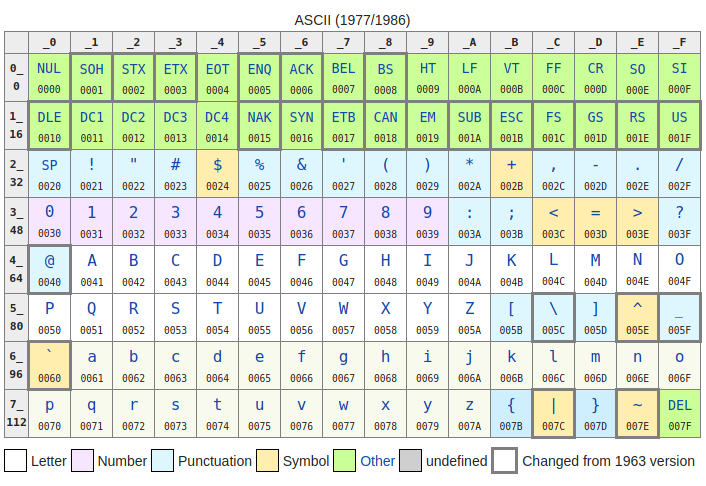
\includegraphics[width=6cm]{img/ascii.png}

  $0, \ldots, 31$ + $127$ $\rightarrow$ non-printable chars (null, new line, tab, others)
  
  $32, \ldots, 126$ $\rightarrow$ printable chars (letters, digits, punctuation, others)
  
  \medskip
  
  Extended ASCII $\rightarrow$ char encoded in 8 bit (add 128 printable chars to standard ASCII)
\end{frame}

%%%%%%%%%%%%%%%%%%%%%%%%%%%%%%%%%%%%%%%%%%%%%%%%%%%%%%%%%%%%%%%%%%%%%%%%%%%%%%%
\begin{frame}{Unicode encoding}

\centering

Obviously 128 (or 256) characters are not enough!\\
(Chinese, cyrillic, greek alphabets, emojis...)

\medskip

Different standards: UTF-8, UTF-16, UTF-32 and others

\medskip


\includegraphics[width=8cm]{img/unicode.png}

\medskip

Currently assigned "only" 137993 characters

\end{frame}

%%%%%%%%%%%%%%%%%%%%%%%%%%%%%%%%%%%%%%%%%%%%%%%%%%%%%%%%%%%%%%%%%%%%%%%%%%%%%%%
\begin{frame}{Morse code}

\centering

(Audio) character encoding scheme used in (telegraph) telecommunication.

\smallskip

Each character is encoded using a combination of short and long signal.

\medskip

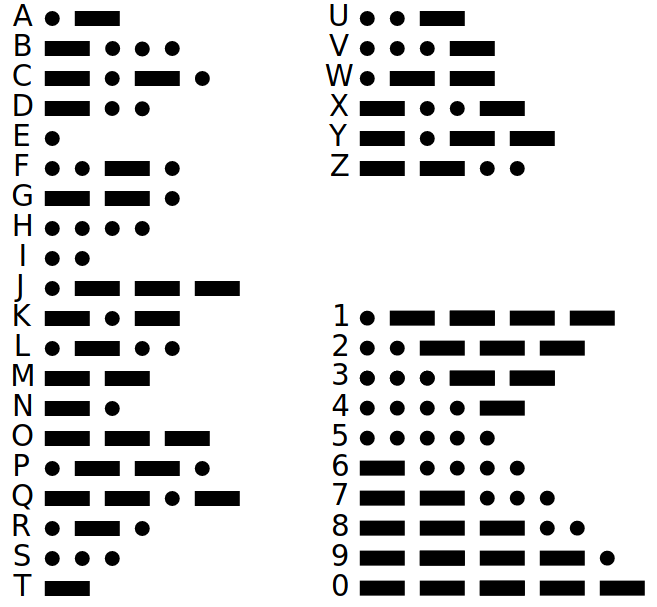
\includegraphics[width=5cm]{img/morse.png}

\end{frame}

%%%%%%%%%%%%%%%%%%%%%%%%%%%%%%%%%%%%%%%%%%%%%%%%%%%%%%%%%%%%%%%%%%%%%%%%%%%%%%%
\begin{frame}{Braille code}

\centering

(Tactile) character encoding scheme used for visually impaired people.

\smallskip

Each characted is encoded using a $2 \times 3$ rectangle with "raised dots".

\medskip

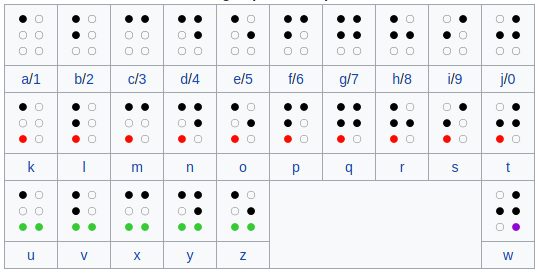
\includegraphics[width=8cm]{img/braille.png}

\end{frame}

%%%%%%%%%%%%%%%%%%%%%%%%%%%%%%%%%%%%%%%%%%%%%%%%%%%%%%%%%%%%%%%%%%%%%%%%%%%%%%%
\begin{frame}{Base64}

  \centering

  Group message in blocks of $6$ bits.

  Advantage: encode all the ASCII chars in printable chars
  
  \smallskip
  
  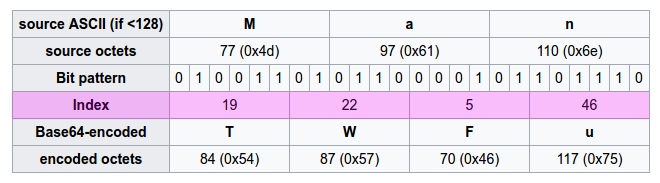
\includegraphics[width=8cm]{img/base64.png}

  \smallskip

  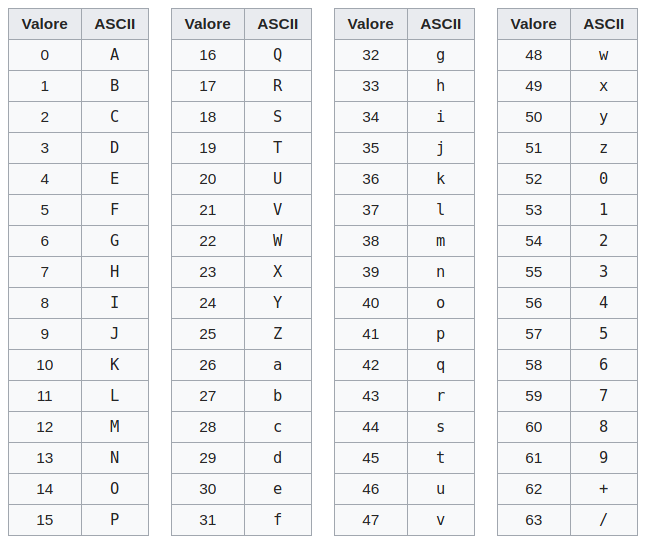
\includegraphics[width=4cm]{img/base64-2.png}

  \smallskip
  
  Message are padded with \textcolor{red}{=} (e.g. \textit{flag} $\rightarrow$ \textit{ZmxhZwo=})
  
\end{frame}

%%%%%%%%%%%%%%%%%%%%%%%%%%%%%%%%%%%%%%%%%%%%%%%%%%%%%%%%%%%%%%%%%%%%%%%%%%%%%%%
%\begin{frame}{Base65536}

%\end{frame}
